\documentclass[conference]{IEEEtran}
\IEEEoverridecommandlockouts
% The preceding line is only needed to identify funding in the first footnote. If that is unneeded, please comment it out.
\usepackage{cite}
\usepackage{amsmath,amssymb,amsfonts}
\usepackage{algorithmic}
\usepackage{graphicx}
\usepackage{textcomp}
\usepackage{xcolor}
\usepackage{url}
\begin{document}

\title{Artificial Creativity}

\author{\IEEEauthorblockN{Federico Matteoni}
\IEEEauthorblockA{\textit{Intelligent Systems for Pattern Recognition} \\
A.Y. 2022/2023 \\
Mat. 530257}
}

\maketitle

\begin{abstract}
This work is a survey on some common machine learning systems aimed at image generation that surfaced in the last years. These systems have recently been used by the general public in viral fashion to generate artistic content, ranging from artistic repropositions of submitted photos to completely new concepts produced by text-based prompts. Although exceptional, these systems also raised some concerns regarding copyright and intellectual property.
\end{abstract}

\section{Introduction}
In January 2021, OpenAI labs presented DALL-E \cite{dallepaper}, a text-to-image generative autoregressive transformer, followed by an unofficial demo. In that demo, users could simply type a text prompt and after few moments a small selection of artistic interpretations of that prompt would be presented. While not being the first text-to-image machine learning model to be presented, it can be argued that DALL-E is the first that had a big impact on the public: in the following months many examples of images generated with that tool would be posted on social media, and many more sophisticated models would surface, taking advantage of the increasing interest in the image generation and \textit{artificial creativity} field.\\
Many of the most recent and successful of these systems stem from the "Diffusion Probabilistic Models" \cite{diffusionmodels} family of machine learning approaches, while some of the earliest examples are Generative Adversarial Networks \cite{GANs} with alternative techniques for the sample generation \cite{stylegan} compared to the classical GAN approaches.
\section{Models}
Image generation, and broadly speaking every kind of data generated through machine learning, is achieved with a family of models called "Generative Models". These models, in contrast with the family of "Discriminative Models", aim to generate new samples of data after learning its distribution, while the goal of discriminative models is to distinguish between different samples of data. Mathematically speaking, given a set of samples $X$ and the corresponding labels $Y$, a generative model learns $p(X, Y)$ while a discriminative model learns $p(X\:|\:Y)$. Generative models can be explicit, when they directly learn $p(X)$, or implicit, if they learn how to sample from $p(X)$ without directly learning it.\\
Text-to-image generation can be achieved with many different kinds of generative models, but we will focus on three main family of models that recently achieved the best results: Generative Adversarial Networks, Autoregressive Transformers and Diffusion Models.
\subsection{Generative Adversarial Networks}
A Generative Adversarial Network (GAN) \cite{GANs} is composed of two main parts: \begin{list}{-}{}
	\item A Generator $\mathcal{G}$ that learns to generate plausible data with the goal of confusing the discriminator
	\item A Discriminator $\mathcal{D}$ that learns to distinguish between the real data and the fake data, penalizing the generator when it produces non-plausible samples
\end{list}
The trick that GANs employ to be able to sample data from complex, high-dimensional distributions, is to sample from a very simple distribution (usually a Gaussian, $\mathcal{N}(0, 1)$) and to train a differentiable distribution (usually a Neural Network, $\mathcal{G}$) to transform the sampled random noise into data from the target distribution: \begin{list}{-}{}
	\item Sample $z\sim\mathcal{N}(0,1)$
	\item Generate $x=\mathcal{G}(z)$
	\item Discriminate $\mathcal{D}(x) = \mathcal{D}(\mathcal{G}(z))$
\end{list}
Given real data $x$ and random noise $z\sim\mathcal{N}(0,1)$, the objective function of a GAN is $C$ defined in \eqref{GANloss}
\begin{equation}
C = \min_\mathcal{G}\max_\mathcal{D}\left( \mathbb{E}_x[\log\mathcal{D}(x)] -\mathbb{E}_z[\log (1-\mathcal{D}(\mathcal{G}(z)))] \right) \label{GANloss}
\end{equation}
This represents a hard two-player game, where the optimal solution resides in a saddle point that corresponds to the concurrent $\min\max$.\\
Most of the works that employ GANs for data generation focus on developing different strategies that adapt the general architecture of these models to the interested data domain. Among the first examples of image generations that reached the general public is thispersondoesnotexist.com, a website published by nVidia which employs a particular GAN architecture, called StyleGAN, to generate highly realistic human portraits. Released in December 2018 with StyleGAN \cite{stylegan} and updated in December 2019 with StyleGAN2 \cite{stylegan2}, this project may represent the first impact that the general public had with state-of-the-art automatic image generation via machine learning models.\\
The original motivation behind StyleGAN was to unbox and better understand the image synthesis process and the properties of the latent spaces employed by the GANs, to both better control the generative process and to better compare different generators between each other. By taking inspiration from the style-transfer literature \cite{styletransfer}, which studies techniques of merging the content of an image with the artistic style of another, the StyleGAN proposed a redesigned generative process: the input latent code (random noise) $z$ is mapped into an intermediate latent space $\mathcal{W}$ which is used to control the generator $\mathcal{G}$ at each layer together with added Gaussian noise. This is in contrast to traditional generators, which feed the input directly to the generating network thus using the latent data just in the input layer. StyleGAN uses latent data to control the generative process at each layer, with $\mathcal{W}$ fed via adaptive instance normalization (AdaIN, \eqref{adain}): it normalizes each feature map $x_i$ separately given the style $y = (y_s, y_b)$ which is synthesized from $\mathcal{W}$ via learned transformations.
\begin{equation}
\hbox{AdaIN}(x_i, y) = y_{si}\frac{x_i-\mu(x_i)}{\sigma(x_i)} + y_{bi}
\label{adain}
\end{equation} 
A main difference from classical style transfer \cite{styletransfer} is that the style $y$ of the target image is computed from $\mathcal{W}$, the latent data, instead of an example image.\\
The noise which is fed independently to each layer of the generative process is used to generate stochastic detail in the final images: these details range from the placement of the skin pores to other details like freckles and hair. By using random noise at each layer the network does not need to use activations from the previous layer, thus reusing data from the only source of input available, to generate stochastic effects: this reduces the occurrence of repetitive patterns, which can be particularly perceivable in the case of human faces. According to style transfer literature, the style of an image is reliably encoded by spatially invariant statistics like channel-wise mean or variance etc., and in StyleGAN the globally defined style affects global effects like lightning, pose and the like, while locally defined noise added independently to each pixel is only used to generate stochastic variation: if the generator tried to control a global effect, e.g. pose, with the noise, this would lead to spatially inconsistent decisions and then penalization by the discriminator. So the network learns to use global and local channels appropriately without explicit guidance, fully employing the power of the adversarial process.\\
Besides thispersondoesnotexists, StyleGANs have been used in other online demos like thisartworkdoesnotexists and thiscatdoesnotexists: an example of the latter is Fig. \ref{styleganimage}.
\begin{figure}[htbp]
\centerline{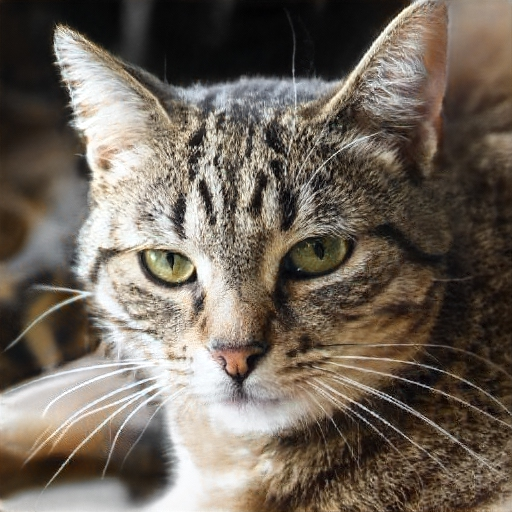
\includegraphics[scale=.33]{img/stylegan.jpg}}
\caption{A cat portrait generated by a StyleGAN.}
\label{styleganimage}
\end{figure}
\subsection{Autoregressive Transformers}
Transformers \cite{transformer} are models that make extensive use of the Attention mechanism \cite{attention}. Attention is a technique that enhances small portions of the input data that are deemed important depending on the context. Given $h_i$ as input, e.g. tokens of latent information, and context information $S$, in its simplest form an attention module computes $C$ in three passes:
\begin{list}{-}{}
	\item Relevance, where each encoding $h_i$ is fused with current context $S$ yielding the relevance $\eta_i$ between the two
	\begin{equation}
	\eta_i = \tanh(S, h_i)
	\label{attentionrelevance}
	\end{equation}
	\item Normalization via a softmax operator
	\begin{equation}
	\alpha_i = \frac{e^{\eta_i}}{\sum_j e^{\eta_j}}
	\label{attentionnormalization}
	\end{equation}
	\item Aggregation by soft attention voting
	\begin{equation}
	C = \sum_i\alpha_ih_i
	\label{attentionaggregation}
	\end{equation}
\end{list}
Transformers are pure attention models with no recurrence that employs a variant of the attention mechanism called self-attention, used to draw global dependencies of the data. Self-attention maps each input to a set of three vectors, called Query (Q), Key (K) and Value (V): these vectors are used to compute the output vector, which is a weighted sum of the Vs where the weights are computed through a compatibility function of the Q and the corresponding K. The version used traditionally in the Transformers is called Scaled Dot-Product Attention, in Eq. \ref{selfatteq} where $d_k$ is the dimension of Q and K.
\begin{equation}
\hbox{Attention}(Q, K, V) = \hbox{Softmax}\left(\frac{QK^T}{\sqrt{d_k}}\right)V
\label{selfatteq}
\end{equation}
A Transformer is made of an encoder and a decoder, both composed by stack of self-attention and fully connected layers. In particular, Autoregressive Transformers use the previous output as an additional input for subsequent passes through the network.\\
DALL-E \cite{dallepaper} is an autoregressive transformer that models the prompt text and image as a single stream of tokens. In order to not use pixels directly as image tokens, and to prevent that much of the modeling capacity is spent capturing high-frequency details (like the stochastic variations of the displacement of hairs and freckles) rather than low-frequency details (like pose and lightning), the training is split into two stages \cite{dallepaper}:
\begin{list}{-}{}
	\item A Discrete Variational Autoencoder (dVAE) is used to compress the images into a grid of tokes, each with 8192 possible values
	\item Up to 256 text tokens are concatenated with the 1024 image tokens to train an autoregressive transformer, that models the joint distribution over the text and image tokens.
\end{list}
The training is performed by maximizing the ELBO of the joint likelihood of the model distribution over images $x$, captions $y$ and tokens $z$ of the encoded image. By factorizing the distribution with $p_{\theta\psi}(x,y,z)=p_\theta(x\:|\:y,z)p_\psi(y,z)$ we have the following lower bound:
\begin{equation}
\begin{aligned}
\ln p_{\theta\psi}(x,y) \geq&\: \mathbb{E}_{z\sim q_\phi(z\:|\:x)}[\ln p_\theta(x\:|\:y,z)-\\
&\:\beta KL(q_\phi(y,z\:|\:x)\:||\:p_\psi(y,z))]
\label{dallelowerbound}
\end{aligned}
\end{equation}
Where $q_\phi$ is the distribution over the images tokes generated by the dVAE given the image, $p_\theta$ is the distribution over the images generated by the decoder given the tokens, $p_\psi$ is the joint distribution over the text and image tokes modeled by the transformer.\\
The resulting model, called DALL-E and shown in Fig. \ref{dalleimage}, has been presented in January 2021 \cite{dalle} and gained online relevance as soon as it came out thanks to a unofficial open-source version formerly called DALL-E mini \cite{dallemini} of which an example of the latest version, called Craiyon, is Fig. \ref{dalleminiimage}.\\
Much of the success that DALL-E faced since its presentation came from the many social media communities that used the tool to quickly generate and share memes, creating a viral phenomenon that contributed to an increased interest in text-to-image models research and in general in the artistic applications of machine learning models.
\begin{figure}[htbp]
\centerline{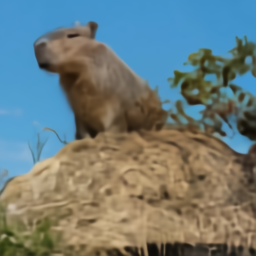
\includegraphics[scale=.6]{img/dalle.png}}
\caption{"A low-angle view of a capybara sitting on a mountain" by DALL-E}
\label{dalleimage}
\end{figure}
\begin{figure}[htbp]
\centerline{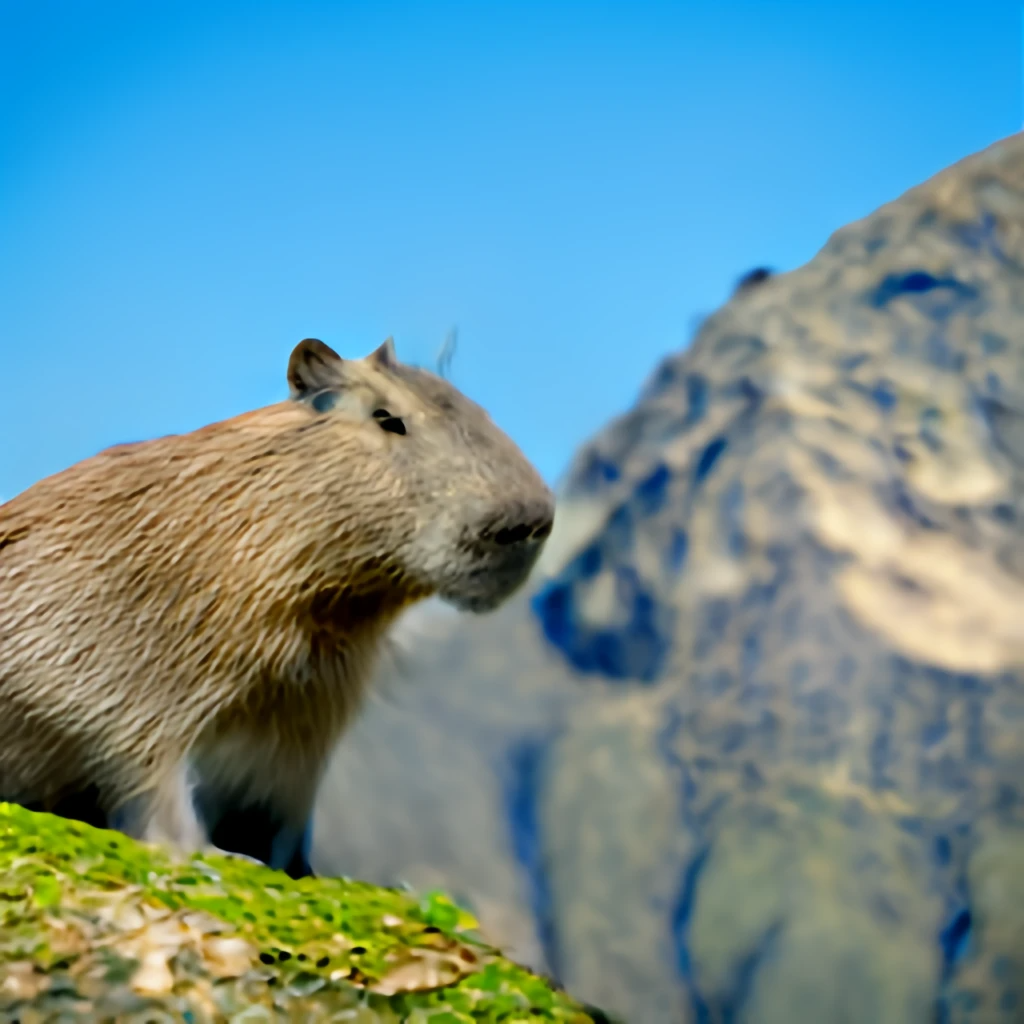
\includegraphics[scale=.15]{img/dallemini.png}}
\caption{"A low-angle view of a capybara sitting on a mountain" by Crayion}
\label{dalleminiimage}
\end{figure}
\subsection{Diffusion Probabilistic Models}
One of the main limitations of machine learning, regarding generative models in particular, is the tractability of the probability distributions involved. Learning, sampling and evaluation are often still analytically or computationally intractable when using highly flexible families of models, thus requiring a tradeoff between these two conflicting goals: flexibility and tractability. Diffusion Probabilistic Models (DM) \cite{diffusionmodels} aim to achieve both, by taking inspiration from statistical physics.\\
DMs are built by two main processes:
\begin{list}{-}{}
	\item A Diffusion Process which converts any complex data distribution into a simple one (e.g. a Gaussian)
	\item A Reverse Process which defines the generative model
\end{list}
The diffusion process gradually converts an input data distribution $q(x^{(0)})$ into a tractable distribution $p(y)$ by repeated application of a Markov Diffusion Kernel \eqref{MarkovDiffusionKernel} where $\beta$ is the diffusion rate
\begin{equation}
T_p(y\:|\:y';\beta)
\label{MarkovDiffusionKernel}
\end{equation}

\begin{equation}
p(y)=\int T_p(y\:|\:y';\beta)p(y')\:dy'
\label{dpmpy}
\end{equation}
\begin{equation}
q\left(x^{(t)}\:|\:x^{(t-1}\right) = T_p\left(x^{(t)}\:|\:x^{(t-1)};\beta\right)
\label{dpmqx}
\end{equation}
The forward trajectory corresponds to performing $T$ steps of diffusion starting from the data distribution and is defined in \eqref{dpmforward}, which exhibits clear Markovian dynamics showing a prior and a first-order transition
\begin{equation}
q\left(x^{(0\ldots T)}\right)=q\left(x^{(0)}\right)\prod^T_{t=1}q\left(x^{(t)}\:|\:x^{(t-1)}\right)
\label{dpmforward}
\end{equation}
The forward diffusion kernel $q\left(x^{(t)}\:|\:x^{(t-1)}\right)$ for example may correspond to a Gaussian Diffusion into a Gaussian distribution with identity covariance, defined in \eqref{forwarddiffusiongaussian}
\begin{equation}
q\left(x^{(t)}\:|\:x^{(t-1)}\right) = \mathcal{N}\left(x^{(t-1)}\sqrt{1-\beta_t},\:\mathbf{I}\beta_t\right)
\label{forwarddiffusiongaussian}
\end{equation}
The generative distribution is trained to describe the same trajectory of the forward process but in reverse, thus yielding the reverse process described in \eqref{dpmreverse}
\begin{equation}
p\left(x^{(0\ldots T)}\right)=p\left(x^{(T)}\right)\prod^T_{t=1}p\left(x^{(t-1)}\:|\:x^{(t)}\right)
\label{dpmreverse}
\end{equation}
During learning, and in the Gaussian diffusion kernel scenario taken as example, only the mean and covariance of the kernel need to be estimated:
\begin{list}{-}{}
	\item $f_\mu(x^{(t)}, t)$ defines the mean of the reverse Markov transitions
	\item $f_\sigma(x^{(t)}, t)$, defines the covariance of the reverse Markov transitions
\end{list}
Both can be defined via neural networks or other function fitting technique and the cost of these functions defines the computational cost of the overall algorithm. Those are used in the reverse diffusion kernel defined in \eqref{reverseduiffusiongaussian}
\begin{equation}
p\left(x^{(t-1)}\:|\:x^{(t)}\right)=\mathcal{N}\left(f_\mu(x^{(t)},t),\:f_\sigma(x^{(t)},t)\right)
\label{reverseduiffusiongaussian}
\end{equation}
The main limitation of classical DMs is that they operate directly in pixel space and require the sequential run of a large number of steps of the Markov chain, thus resulting in expensive and long optimization (e.g. 150-1000 GPU days \cite{gpudays}) and inference processes (circa 5 days to produce 50k images \cite{gpudays}). This has multiple consequences, beginning with the carbon footprint, the unavailability of such computational resources to many researchers and the unapplicability of these models to real-word scenarios.\\
To increase the accessibility of these models, the Latent Diffusion Model (LDM) \cite{latentdiffusionpaper} family of approaches have been proposed. These models split training into two distinct phases:
\begin{list}{-}{}
	\item Train an Autoencoder \cite{autoencoders} that provides a lower-dimensional representational space, more efficient than pixel space and perceptually equivalent
	\item Train the DM in the learned latent, smaller and more efficient, space
\end{list}
The resulting model, a LDM, exhibits better scaling properties and more efficient image generation than traditional DMs. A notable advantage is that the autoencoder may need to be trained just once, and then be used for multiple different LDMs or for completely different models.\\
A successful application of LDMs is the Stable Diffusion model \cite{stablediffusionesource} released in 2022, an open source implementation of an LDMs trained on the LAION-5B dataset \cite{laion5b}. This model has been used in several projects \cite{stablediffusionprojects} and in a online demo \cite{stablediffusiondemo}: an example of an image generated by this demo is Fig. \ref{ldmimage}. Another notable example is Midjourney \cite{midjourney}, released in 2022 as well, a commercial application of a DM with the goal of being a tool for artists. An example of an image produced by Midjourney is Fig. \ref{midjourneyimage}.\\
LDMs recently have been implemented in mobile apps, highlighting their generation efficiency and general-purpose. This is one of the main differences between GANs (e.g. StyleGAN) and DMs (e.g. Stable Diffusion), with the first achieving great result only on data with limited variability with an overall small flexibility, while the latter showing more flexibility.
\begin{figure}[htbp]
\centerline{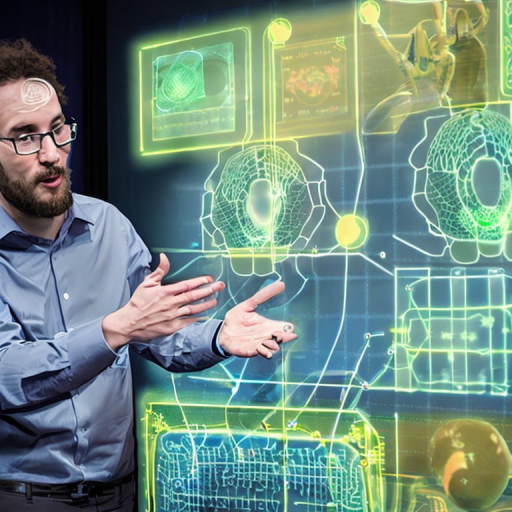
\includegraphics[scale=.4]{img/stablediffusion.jpg}}
\caption{"A teacher explaining artificial intelligence with holograms" by Stable Diffusion 2.1}
\label{ldmimage}
\end{figure}
\begin{figure}[htbp]
\centerline{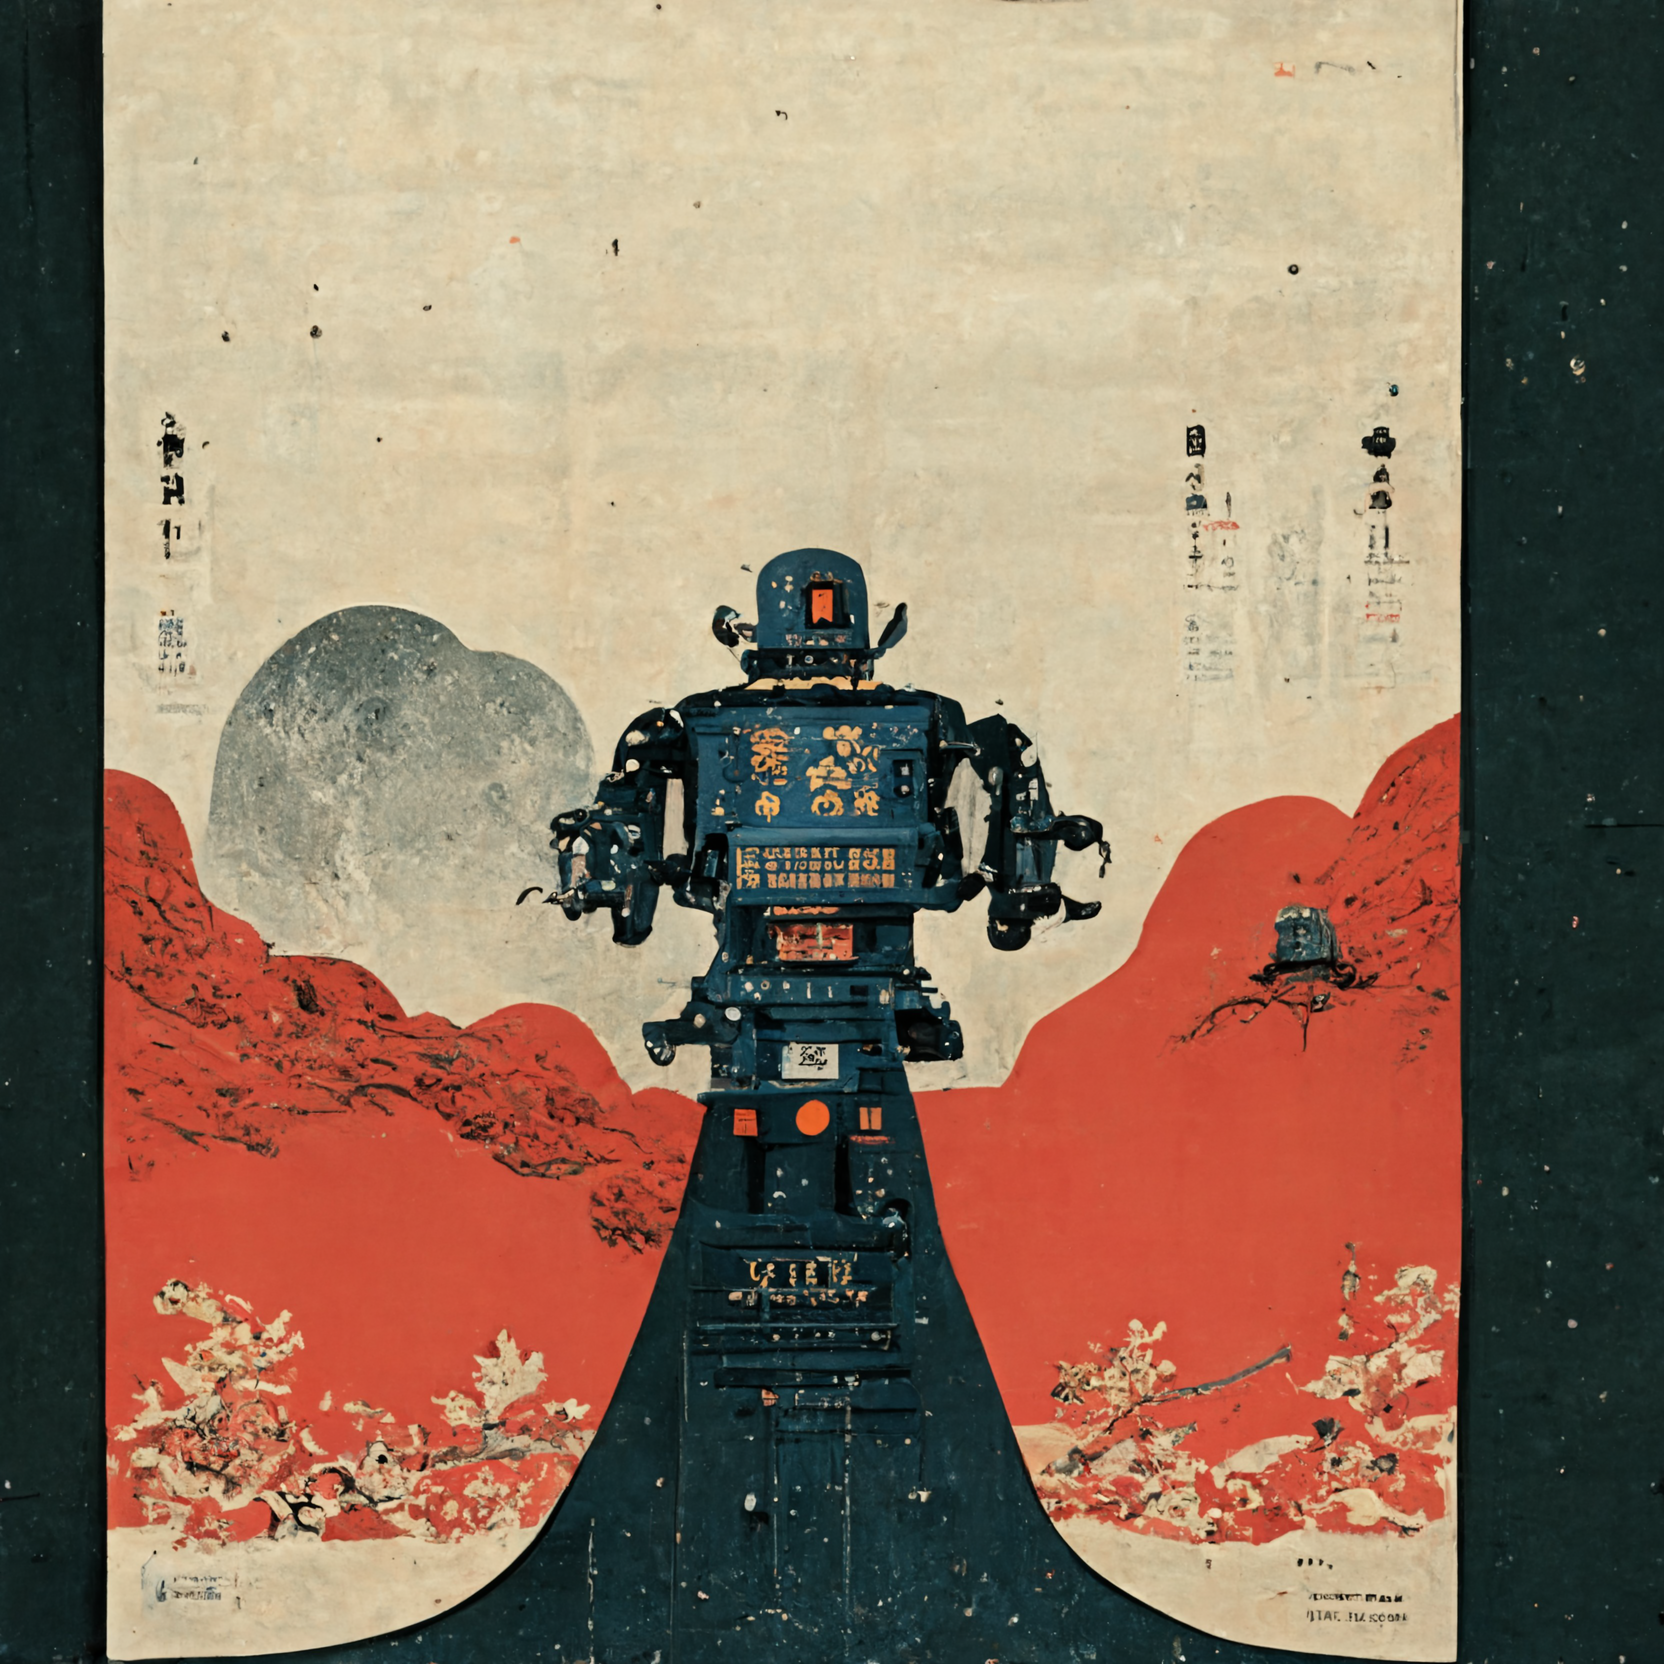
\includegraphics[scale=.09]{img/midjourney/fexed_ukiyo-e_robot_detailed_449ecbde-e204-4e21-8542-9c40ef906080.png}}
\caption{"Ukiyo-e, robot, detailed" by Midjourney}
\label{midjourneyimage}
\end{figure}
\section{Datasets}
In just few years, from models capable of generating high quality samples from a specific domain like human portraits or cats, we now have models that are capable of generating arbitrary images starting from a simple text prompt and in just few moments. Aside from the novel ideas and solutions regarding training and generation, very important contributors of this fast improvement are the datasets on which the models have been trained.
\subsection{LAION}
LAION-400M \cite{laion400m}, released in 2021, and its newest version LAION-5B \cite{laion5b}, released in 2022, are openly available datasets composed by image-text pairs. Massive datasets, like the one used to train GPT-3 or to scale up various models, are rarely released publicly maybe due to industrial secret or legal reasons. LAION-400M was initially released in order to address this issue, by providing a curated and filtered massive dataset in order to push forward the research involving these data. LAION-5B contains more than 5 billion image-text pairs, for a total of 240 terabytes of data. It also provides kNN indices to speed up search, tools for building the dataset, subset of the datasets useful for testing or more focused tasks and other metadata. LAION datasets are built through a post-processing of data contained in the Common Crawl dataset.
\subsection{Common Crawl}
Common Crawl \cite{commoncrawl} is a corpus containing petabytes of data collected since 2008, composed by raw web pages, metadata and text. Its access is completely free. It works via a bot, now called CCBot/2.0, that scrapes the web, accesses each webpage identifying itself and gathers the data it needs. The data is then stored in servers which, where is processed and archived in the WARC format. 
%
% NOTE
% Considerazioni finali riguardo: necessità di invisible watermarking (https://github.com/ShieldMnt/invisible-watermark)

% CHARGPT
%I am a large language model trained by OpenAI. Language models are trained to predict the next word in a sequence of words, based on the context of the words that come before it. This allows me to understand and generate human-like text.
%I was trained on a dataset of more than 8 million web pages, including articles, books, and websites. This dataset was used to teach me the structure and conventions of the English language, as well as the relationships between words and the meanings they convey.
%I am able to understand and generate text in a wide range of styles and formats, including conversational language, technical language, and creative language. I am also able to understand and respond to user input in a natural and intuitive way, by considering the context and intent behind the words that are used.
%I am constantly learning and adapting to new information, and I am able to provide accurate and up-to-date information on a wide range of topics. However, it is important to note that my knowledge is limited to what was available at the time of my training, and I am not able to browse the internet or access new information.

\iffalse
\section{Ease of Use}

\subsection{Maintaining the Integrity of the Specifications}

The IEEEtran class file is used to format your paper and style the text. All margins, 
column widths, line spaces, and text fonts are prescribed; please do not 
alter them. You may note peculiarities. For example, the head margin
measures proportionately more than is customary. This measurement 
and others are deliberate, using specifications that anticipate your paper 
as one part of the entire proceedings, and not as an independent document. 
Please do not revise any of the current designations.

\section{Prepare Your Paper Before Styling}
Before you begin to format your paper, first write and save the content as a 
separate text file. Complete all content and organizational editing before 
formatting. Please note sections \ref{AA}--\ref{SCM} below for more information on 
proofreading, spelling and grammar.

Keep your text and graphic files separate until after the text has been 
formatted and styled. Do not number text heads---{\LaTeX} will do that 
for you.

\subsection{Abbreviations and Acronyms}\label{AA}
Define abbreviations and acronyms the first time they are used in the text, 
even after they have been defined in the abstract. Abbreviations such as 
IEEE, SI, MKS, CGS, ac, dc, and rms do not have to be defined. Do not use 
abbreviations in the title or heads unless they are unavoidable.

\subsection{Units}
\begin{itemize}
\item Use either SI (MKS) or CGS as primary units. (SI units are encouraged.) English units may be used as secondary units (in parentheses). An exception would be the use of English units as identifiers in trade, such as ``3.5-inch disk drive''.
\item Avoid combining SI and CGS units, such as current in amperes and magnetic field in oersteds. This often leads to confusion because equations do not balance dimensionally. If you must use mixed units, clearly state the units for each quantity that you use in an equation.
\item Do not mix complete spellings and abbreviations of units: ``Wb/m\textsuperscript{2}'' or ``webers per square meter'', not ``webers/m\textsuperscript{2}''. Spell out units when they appear in text: ``. . . a few henries'', not ``. . . a few H''.
\item Use a zero before decimal points: ``0.25'', not ``.25''. Use ``cm\textsuperscript{3}'', not ``cc''.)
\end{itemize}

\subsection{Equations}
Number equations consecutively. To make your 
equations more compact, you may use the solidus (~/~), the exp function, or 
appropriate exponents. Italicize Roman symbols for quantities and variables, 
but not Greek symbols. Use a long dash rather than a hyphen for a minus 
sign. Punctuate equations with commas or periods when they are part of a 
sentence, as in:
\begin{equation}
a+b=\gamma\label{eq}
\end{equation}

Be sure that the 
symbols in your equation have been defined before or immediately following 
the equation. Use ``\eqref{eq}'', not ``Eq.~\eqref{eq}'' or ``equation \eqref{eq}'', except at 
the beginning of a sentence: ``Equation \eqref{eq} is . . .''

\subsection{\LaTeX-Specific Advice}

Please use ``soft'' (e.g., \verb|\eqref{Eq}|) cross references instead
of ``hard'' references (e.g., \verb|(1)|). That will make it possible
to combine sections, add equations, or change the order of figures or
citations without having to go through the file line by line.

Please don't use the \verb|{eqnarray}| equation environment. Use
\verb|{align}| or \verb|{IEEEeqnarray}| instead. The \verb|{eqnarray}|
environment leaves unsightly spaces around relation symbols.

Please note that the \verb|{subequations}| environment in {\LaTeX}
will increment the main equation counter even when there are no
equation numbers displayed. If you forget that, you might write an
article in which the equation numbers skip from (17) to (20), causing
the copy editors to wonder if you've discovered a new method of
counting.

{\BibTeX} does not work by magic. It doesn't get the bibliographic
data from thin air but from .bib files. If you use {\BibTeX} to produce a
bibliography you must send the .bib files. 

{\LaTeX} can't read your mind. If you assign the same label to a
subsubsection and a table, you might find that Table I has been cross
referenced as Table IV-B3. 

{\LaTeX} does not have precognitive abilities. If you put a
\verb|\label| command before the command that updates the counter it's
supposed to be using, the label will pick up the last counter to be
cross referenced instead. In particular, a \verb|\label| command
should not go before the caption of a figure or a table.

Do not use \verb|\nonumber| inside the \verb|{array}| environment. It
will not stop equation numbers inside \verb|{array}| (there won't be
any anyway) and it might stop a wanted equation number in the
surrounding equation.

\subsection{Some Common Mistakes}\label{SCM}
\begin{itemize}
\item The word ``data'' is plural, not singular.
\item The subscript for the permeability of vacuum $\mu_{0}$, and other common scientific constants, is zero with subscript formatting, not a lowercase letter ``o''.
\item In American English, commas, semicolons, periods, question and exclamation marks are located within quotation marks only when a complete thought or name is cited, such as a title or full quotation. When quotation marks are used, instead of a bold or italic typeface, to highlight a word or phrase, punctuation should appear outside of the quotation marks. A parenthetical phrase or statement at the end of a sentence is punctuated outside of the closing parenthesis (like this). (A parenthetical sentence is punctuated within the parentheses.)
\item A graph within a graph is an ``inset'', not an ``insert''. The word alternatively is preferred to the word ``alternately'' (unless you really mean something that alternates).
\item Do not use the word ``essentially'' to mean ``approximately'' or ``effectively''.
\item In your paper title, if the words ``that uses'' can accurately replace the word ``using'', capitalize the ``u''; if not, keep using lower-cased.
\item Be aware of the different meanings of the homophones ``affect'' and ``effect'', ``complement'' and ``compliment'', ``discreet'' and ``discrete'', ``principal'' and ``principle''.
\item Do not confuse ``imply'' and ``infer''.
\item The prefix ``non'' is not a word; it should be joined to the word it modifies, usually without a hyphen.
\item There is no period after the ``et'' in the Latin abbreviation ``et al.''.
\item The abbreviation ``i.e.'' means ``that is'', and the abbreviation ``e.g.'' means ``for example''.
\end{itemize}
An excellent style manual for science writers is \cite{b7}.

\subsection{Authors and Affiliations}
\textbf{The class file is designed for, but not limited to, six authors.} A 
minimum of one author is required for all conference articles. Author names 
should be listed starting from left to right and then moving down to the 
next line. This is the author sequence that will be used in future citations 
and by indexing services. Names should not be listed in columns nor group by 
affiliation. Please keep your affiliations as succinct as possible (for 
example, do not differentiate among departments of the same organization).

\subsection{Identify the Headings}
Headings, or heads, are organizational devices that guide the reader through 
your paper. There are two types: component heads and text heads.

Component heads identify the different components of your paper and are not 
topically subordinate to each other. Examples include Acknowledgments and 
References and, for these, the correct style to use is ``Heading 5''. Use 
``figure caption'' for your Figure captions, and ``table head'' for your 
table title. Run-in heads, such as ``Abstract'', will require you to apply a 
style (in this case, italic) in addition to the style provided by the drop 
down menu to differentiate the head from the text.

Text heads organize the topics on a relational, hierarchical basis. For 
example, the paper title is the primary text head because all subsequent 
material relates and elaborates on this one topic. If there are two or more 
sub-topics, the next level head (uppercase Roman numerals) should be used 
and, conversely, if there are not at least two sub-topics, then no subheads 
should be introduced.

\subsection{Figures and Tables}
\paragraph{Positioning Figures and Tables} Place figures and tables at the top and 
bottom of columns. Avoid placing them in the middle of columns. Large 
figures and tables may span across both columns. Figure captions should be 
below the figures; table heads should appear above the tables. Insert 
figures and tables after they are cited in the text. Use the abbreviation 
``Fig.~\ref{fig}'', even at the beginning of a sentence.

\begin{table}[htbp]
\caption{Table Type Styles}
\begin{center}
\begin{tabular}{|c|c|c|c|}
\hline
\textbf{Table}&\multicolumn{3}{|c|}{\textbf{Table Column Head}} \\
\cline{2-4} 
\textbf{Head} & \textbf{\textit{Table column subhead}}& \textbf{\textit{Subhead}}& \textbf{\textit{Subhead}} \\
\hline
copy& More table copy$^{\mathrm{a}}$& &  \\
\hline
\multicolumn{4}{l}{$^{\mathrm{a}}$Sample of a Table footnote.}
\end{tabular}
\label{tab1}
\end{center}
\end{table}

\begin{figure}[htbp]
\centerline{\includegraphics{fig1.png}}
\caption{Example of a figure caption.}
\label{fig}
\end{figure}

Figure Labels: Use 8 point Times New Roman for Figure labels. Use words 
rather than symbols or abbreviations when writing Figure axis labels to 
avoid confusing the reader. As an example, write the quantity 
``Magnetization'', or ``Magnetization, M'', not just ``M''. If including 
units in the label, present them within parentheses. Do not label axes only 
with units. In the example, write ``Magnetization (A/m)'' or ``Magnetization 
\{A[m(1)]\}'', not just ``A/m''. Do not label axes with a ratio of 
quantities and units. For example, write ``Temperature (K)'', not 
``Temperature/K''.

\section*{Acknowledgment}

The preferred spelling of the word ``acknowledgment'' in America is without 
an ``e'' after the ``g''. Avoid the stilted expression ``one of us (R. B. 
G.) thanks $\ldots$''. Instead, try ``R. B. G. thanks$\ldots$''. Put sponsor 
acknowledgments in the unnumbered footnote on the first page.

\section*{References}

Please number citations consecutively within brackets \cite{b1}. The 
sentence punctuation follows the bracket \cite{b2}. Refer simply to the reference 
number, as in \cite{b3}---do not use ``Ref. \cite{b3}'' or ``reference \cite{b3}'' except at 
the beginning of a sentence: ``Reference \cite{b3} was the first $\ldots$''

Number footnotes separately in superscripts. Place the actual footnote at 
the bottom of the column in which it was cited. Do not put footnotes in the 
abstract or reference list. Use letters for table footnotes.

Unless there are six authors or more give all authors' names; do not use 
``et al.''. Papers that have not been published, even if they have been 
submitted for publication, should be cited as ``unpublished'' \cite{b4}. Papers 
that have been accepted for publication should be cited as ``in press'' \cite{b5}. 
Capitalize only the first word in a paper title, except for proper nouns and 
element symbols.

For papers published in translation journals, please give the English 
citation first, followed by the original foreign-language citation \cite{b6}.

\vspace{12pt}
\color{red}
IEEE conference templates contain guidance text for composing and formatting conference papers. Please ensure that all template text is removed from your conference paper prior to submission to the conference. Failure to remove the template text from your paper may result in your paper not being published.
\fi

\bibliographystyle{plain}
\bibliography{references}
\end{document}
